\documentclass{beamer}
\usepackage[T1]{fontenc}
\usepackage[utf8]{inputenc}
\usepackage{lmodern}
\usepackage{minted}
\usepackage{multicol}
\usepackage{amsmath}

\usetheme{metropolis}

\title{Boosting Distributed Machine Learning System with Application-aware Network Scheduling}
\author{Zheng Luo}

\begin{document}

\begin{frame}
  \titlepage
\end{frame}

\section{Background \& Previous Research}
\begin{frame}{Big Data With SDN}
    Big Data applications\footnotemark:
    \begin{itemize}
        \item Require high bandwidth
        \item Have well-defined computational/traffic patterns
        \item Have a centralized management structure
    \end{itemize}
    
    Therefore, it is possible to leverage application-aware information to improve network scheduling, especially in a software-defined network.
    
    \footnotetext{Programming Your Network at Run-time
for Big Data Applications, HotSDN, Guohui Wang et. al., 2013}
\end{frame}

\begin{frame}{Compared with Our Last Research}
In our last paper \small{\emph{BAHS: A Bandwidth-Aware Heterogeneous Scheduling Approach for SDN-based Cluster Systems}}, we used \emph{network information} to support \emph{task scheduling in Hadoop System}.

What about the reverse?

\begin{quotation}
Big data can also benefit SDN, including traffic engineering, cross-layer design, defeating security attacks, and SDN-based intra- and inter-data-center networks.\footnotemark[1]
\end{quotation}

Why the reverse is better:
\begin{quotation}
Today, application schedules tasks in a network-agnostic way\footnotemark[2]
\end{quotation}

\footnotetext[1]{When big data meets software-defined networking: SDN for big data and big data for SDN, Laizhong Cui et. al., IEEE Journal of Networks, 2016}
\footnotetext[2]{Cross-Layer Scheduling in Cloud Systems, Hilfi Alkaff et. al., IEEE International Conference on Cloud Engineering, 2015}
\end{frame}

\begin{frame}{Application-aware scheduling}
\centering
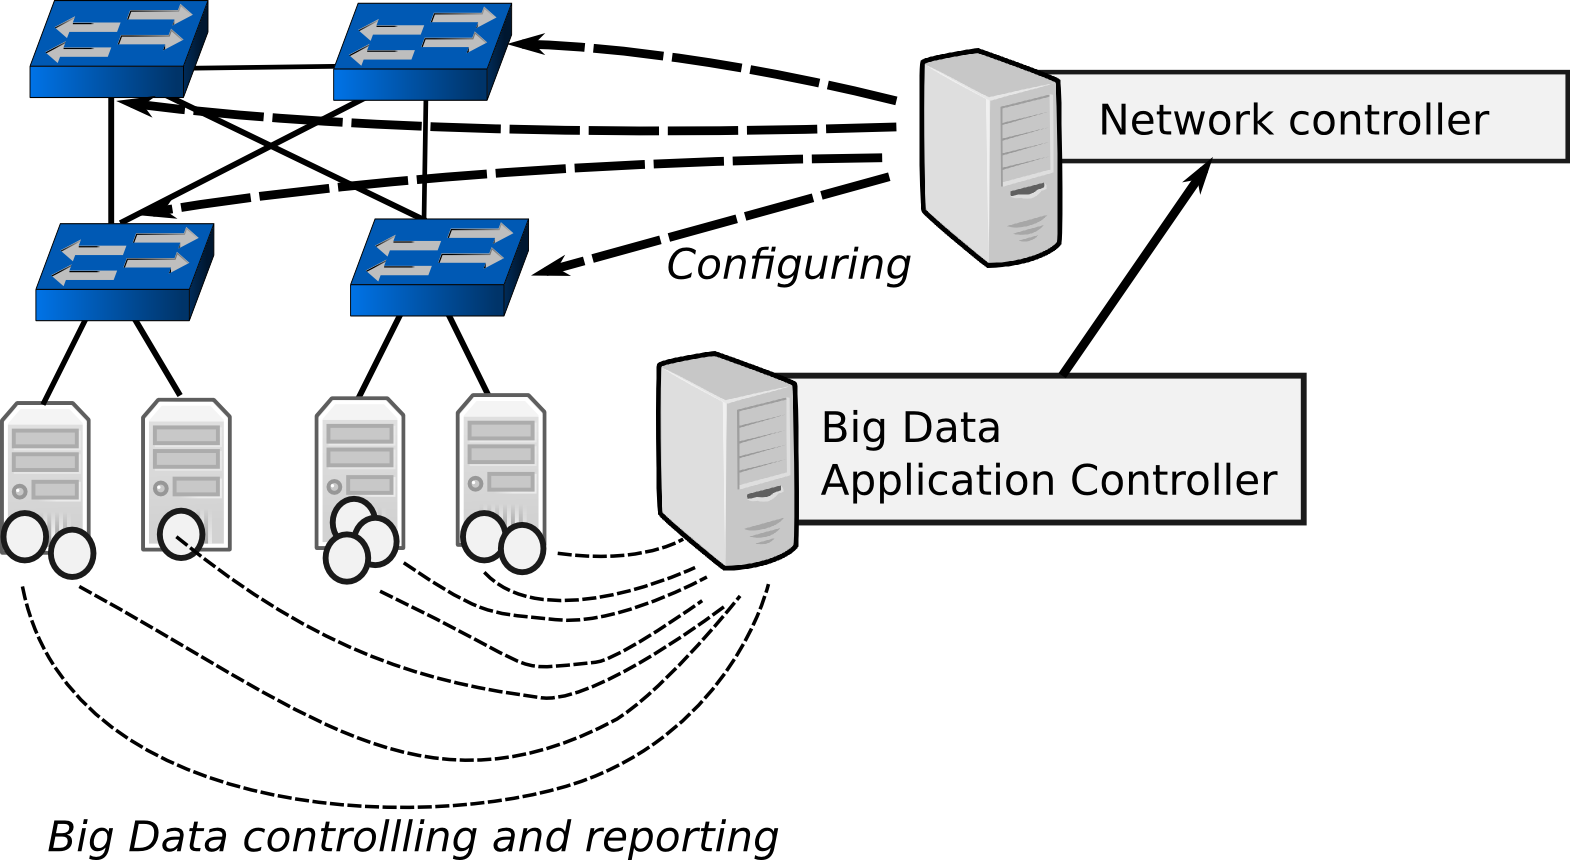
\includegraphics[scale=.15]{application-aware-scheduling.png}\footnotemark

\footnotetext{Network Configuration and Flow Scheduling for Big Data
Applications, Lautaro Dolberg et. al., Networking for Big Data, 2015}
\end{frame}

\begin{frame}{A typical example: HadoopWatch}
HadoopWatch\footnotemark is a typical example to perform such cross-layer network scheduling:

\begin{columns}
    \begin{column}{0.6\linewidth}
        \centering
        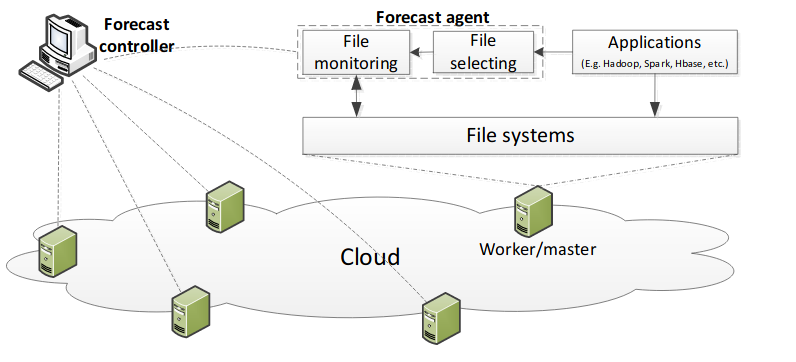
\includegraphics[scale=.23]{hadoopwatch.png}
    \end{column}
    \begin{column}{0.4\linewidth}
        \begin{itemize}
            \item Predict task status by monitoring file system
            \item Calculate task \& flow dependencies
            \item Assign higher priority to slow/blocking flows
        \end{itemize}
    \end{column}
\end{columns}
\footnotetext{HadoopWatch: A first step towards comprehensive traffic forecasting in cloud computing, Yang Peng et. al., INFOCOM, 2014}
\end{frame}

\begin{frame}{After HadoopWatch}
A lot of research on application-aware scheduling conducted on Hadoop, Storm and Flink.

Basically consisting three parts:
\begin{itemize}
    \item Predict flows \& Aggregate multiple flows into an application-level task
    \item Calculate priorities of flows based on application-level information
    \item Change routing configuration on switches to achieve QoS scheduling
\end{itemize}
\end{frame}

\section{Incorperate application-aware scheduling to distributed machine learning}
\begin{frame}{Parameter server architecture}
\begin{columns}
    \begin{column}{0.5\linewidth}
        \centering
        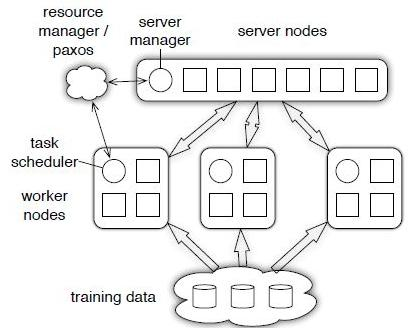
\includegraphics[scale=.35]{parameter-server.jpg}
    \end{column}
    \begin{column}{0.5\linewidth}
        \begin{itemize}
            \item Require high bandwidth? YES. Real-world model contains $10^9$ to $10^{12}$ parameters. \footnotemark
            \item Well-defined patterns? YES. Worker pull parameters from server, and push gradients to server in a batch.
            \item Centralized architecture? YES. Most use a single scheduler.
        \end{itemize}
    \end{column}
\end{columns}

\footnotetext{Scaling Distributed Machine Learning with the Parameter Server, Mu Li et. al., OSDI, 2014}
\end{frame}

\begin{frame}{Proposed methods}
Expect to conduct experiments on Apache MXNet\footnotemark, a widely-used distributed machine learning framework.

Typical workflow for a worker:
\begin{itemize}
    \item (Batch 1) Pull parameter
    \item Calculation
    \item Push gradients to parameter server
    \item (Wait for all other worker to finish batch 1)
    \item (Server updating parameters)
    \item (Batch 2) Pull parameter...
\end{itemize}

\footnotetext{MXNet: A Flexible and Efficient Machine Learning
Library for Heterogeneous Distributed Systems, Tianqi Chen et. al., NIPS LearningSys, 2016}
\end{frame}

\begin{frame}{Proposed methods (2)}

Easy to categorize flows:
\begin{itemize}
    \item pull flow = server to worker
    \item push flow = worker to server
    \item Batch number are explicitly output to worker's logs
     Late batch (=smaller batch number) has higher priority. Pull flows > Push flows in the same batch
\end{itemize}

Easy to determine the priority of flows:
\begin{itemize}
    \item Smaller batch number -> higher priority
    \item Pull flows > push flows in the same batch
\end{itemize}

\end{frame}

\begin{frame}{Proposed architecture}
\centering
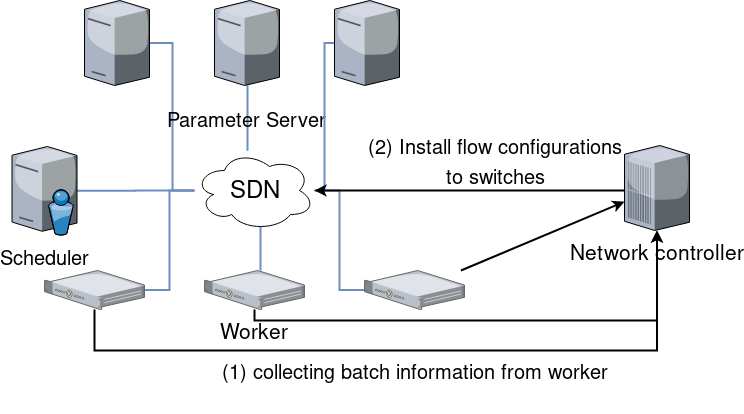
\includegraphics[scale=.3]{ml-sdn-arch.png}
\end{frame}
\end{document}
